\documentclass[10pt, twocolumn, a4paper, fleqn]{article}
\usepackage[italian]{babel}
\usepackage[utf8]{inputenc}
\usepackage{microtype}
\usepackage{hyperref}
\usepackage{indentfirst}
\usepackage[T1]{fontenc}
\usepackage{amsfonts}
\usepackage{amsmath}
\usepackage{amsthm}
\usepackage{amssymb}
\usepackage{array}
\usepackage{booktabs}
\usepackage{braket}
\usepackage{calrsfs}
\usepackage{caption}
\usepackage{multirow}
\usepackage[output-decimal-marker = {.}, exponent-product = \cdot]{siunitx}
\usepackage{pdfpages}
\usepackage{tabularx}
\usepackage{verbatim}

\def\b{\textbf}
\def\bb{\mathbf}
\def\grad{\nabla}
\def\rot{\grad\times}
\def\div{\grad\cdot}
\def\const{\textrm{const}}
\def\sat{\textrm{sat}}
\def\loc{\textrm{loc}}
\def\({\left(}
\def\){\right)}
\def\[{\left[}
\def\]{\right]}

\def\e{\varepsilon}
\def\ke{{\varepsilon_r}}
\def\km{\kappa_m}
\def\chim{\chi_m}
\def\E{\bb{E}}
\def\El{\E_{\textrm{loc}}}
\def\P{\bb{P}}
\def\D{\bb{D}}
\def\F{\bb{F}}
\def\B{\bb{B}}
\def\Bl{\B_{\textrm{loc}}}
\def\H{\bb{H}}
\def\m{\bb{m}}
\def\M{\bb{M}}
\def\j{\bb{j}}
\def\jsm{\bb{j}_{s,m}}
\def\u{\bb{u}}
\def\un{\bb{u}_n}
\def\ut{\bb{u}_t}
\def\ds{ d\bb{s}}
\def\L{\bb{L}}
\def\S{\bb{S}}
\def\J{\bb{J}}
\def\MM{\mathcal{M}}
\def\o{\bb{\omega}}
\def\v{\bb{v}}
\def\I{\bb{I}}
\def\p{\bb{p}}
\def\r{\bb{r}}
\def\k{\bb{k}}
\def\q{\bb{q}}
\def\In{\mathcal{I}}
\def\n{n_}

\def\de{$\e$ }
\def\dke{$\ke$ }
\def\dkm{$\km$ }
\def\dchim{$\chim$ }
\def\dE{$\E$ }
\def\dEl{$\El$ }
\def\dP{$\P$ }
\def\dD{$\D$ }
\def\dF{$\F$ }
\def\dB{$\B$ }
\def\dBl{$\Bl$ }
\def\dH{$\H$ }
\def\dm{$\m$ }
\def\dM{$\M$ }
\def\dj{$\j$ }
\def\djsm{$\jsm$ }
\def\du{$\u$ }
\def\dun{$\un$ }
\def\dut{$\ut$ }
\def\dL{$\L$ }
\def\dS{$\S$ }
\def\dJ{$\J$ }
\def\dMM{$\MM$ }
\def\do{$\omega$ }
\def\dv{$\v$ }
\def\dI{$\I$ }
\def\dr{$\r$ }
\def\dk{$\k$ }
\def\dq{$\q$ }

%\title{Formule di\\ Elettromagnetismo}
%\author{Francesco Dulio}
%\date{}
\begin{document}
%\maketitle
\begin{equation*}\begin{split}
\left[\E\right]=\si{V m^{-1}} \qquad \left[\D\right]=\left[\P\right]=\si{C m^{-2}}
\end{split}\end{equation*}
\begin{equation*}\begin{split}
\left[C\right]=\si{C V^{-1}} \qquad \left[\e_0\right]=\SI{8.85e-12}{F m^{-1}}
\end{split}\end{equation*}

\begin{equation*}\begin{split}
\Phi\left(\E\right)=\frac{q_p}{\e_0}
\end{split}\end{equation*}
\begin{equation*}\begin{split}
\E\left(r\right)=\frac{q}{4\pi\e r^2}\u_r=\frac{\D\left(r\right)}{\e}=\frac{\E_0\left(r\right)}{\ke}
\end{split}\end{equation*}
\begin{equation*}\begin{split}
\E\left(R\right)=\frac{q}{4\pi\e R^2}=\frac{\sigma_0}{\e}\u_r
\end{split}\end{equation*}
\begin{equation*}\begin{split}
\Phi\left(\D\right)=\oint{\D\cdot \un d\Sigma}=q
\end{split}\end{equation*}
\begin{equation*}\begin{split}
\D=\e_0\E+\P=\e\E
\end{split}\end{equation*}
\begin{equation*}\begin{split}
\P\left(r\right)=\frac{\ke-1}{\ke}\D=\e_0\left(\ke-1\right)\E=\frac{\ke-1}{\ke}\sigma_0=\e\chi\E
\end{split}\end{equation*}
\begin{equation*}\begin{split}
\P\left(R\right)=\frac{\ke-1}{\ke}\sigma_0\u_r
\end{split}\end{equation*}
\begin{equation*}\begin{split}
\sigma_p=\P\left(R\right)\cdot \u_r=\frac{\ke-1}{\ke}\sigma_0=\e_0\Delta E=\\
=\sigma_0\left(\frac{\ke_1-\ke_2}{\ke_1\ke_2}\right)=\sigma_1-\sigma_2
\end{split}\end{equation*}
\begin{equation*}\begin{split}
\rho=\nabla \cdot \D
\end{split}\end{equation*}
\begin{equation*}\begin{split}
q_p=-\frac{\ke-1}{\ke}q
\end{split}\end{equation*}
\begin{equation*}\begin{split}
V=\int{\E\cdot d\bb{h}}
\end{split}\end{equation*}
\begin{equation*}\begin{split}
C=\frac{q}{V}
\end{split}\end{equation*}
\begin{equation*}\begin{split}
dU_e=\frac{1}{2}V^2dC
\end{split}\end{equation*}
\begin{equation*}\begin{split}
U_e\left(x\right)=\frac{q^2}{2C}=\int{\frac{1}{2}e\E^2 d\tau}=\int{\frac{1}{2}\frac{\D^2}{\e}d\tau}
\end{split}\end{equation*}

Condensatore piano
\begin{equation*}\begin{split}
\F=\frac{\e_0\rho}{2h}\left(\ke-1\right)V_0^2
\end{split}\end{equation*}

Sfera
\begin{equation*}\begin{split}
\D\left(r\right)=\frac{q}{4\pi r^2}\u_r
\end{split}\end{equation*}
\begin{equation*}\begin{split}
C=4\pi\e R
\end{split}\end{equation*}
\begin{equation*}\begin{split}
\E_c=\left(1-\frac{1}{3}\right)\E
\end{split}\end{equation*}
\begin{equation*}\begin{split}
q_p\left(R\right)=\sigma_p\left(R\right)4\pi R^2
\end{split}\end{equation*}
\begin{equation*}\begin{split}
\p=4\pi\e_0R^3\frac{\ke-1}{\ke-2}\E_0
\end{split}\end{equation*}

Cilindro
\begin{equation*}\begin{split}
\D\left(r\right)=\frac{R}{r}\sigma_0
\end{split}\end{equation*}
\begin{equation*}\begin{split}
\E_c=\E+\frac{\P}{2\e_0}\left[\left(1-\cos{\left(\theta^+\right)}\right)+\left(1-\cos{\left(\theta^-\right)}\right)\right]
\end{split}\end{equation*}
\begin{equation*}\begin{split}
C=\frac{2\pi\e l}{\ln{\left(\frac{R_2}{R_1}\right)}}
\end{split}\end{equation*}

\begin{equation*}\begin{split}
\B=\mu\H=\frac{\mu i}{4\pi}\oint{\frac{\ds\times\u_r}{r^2}}
\end{split}\end{equation*}
\begin{equation*}\begin{split}
\H=\frac{\B}{\mu_0}-\M
\end{split}\end{equation*}
\begin{equation*}\begin{split}
\M=\frac{\m}{\tau}=\chim\H
\end{split}\end{equation*}
\begin{equation*}\begin{split}
i_m=\oint{\M\cdot \ds}
\end{split}\end{equation*}
\begin{equation*}\begin{split}
i=\oint{\H\cdot \ds}
\end{split}\end{equation*}
\begin{equation*}\begin{split}
\j_{s,m}=\M\times\u_n
\end{split}\end{equation*}
\begin{equation*}\begin{split}
\j_{m}=\nabla\times \M
\end{split}\end{equation*}
\begin{equation*}\begin{split}
\j=\nabla \times\H
\end{split}\end{equation*}

Solenoide toroidale
\begin{equation*}\begin{split}
\H=\frac{Ni}{2\pi r}\u_{\phi}
\end{split}\end{equation*}
\begin{equation*}\begin{split}
\B=\frac{\mu Ni}{2\pi r}\u_{\phi}
\end{split}\end{equation*}

Solenoide indefinito
\begin{equation*}\begin{split}
\H=ni\u_z
\end{split}\end{equation*}
\begin{equation*}\begin{split}
\j_m=0 \qquad \j_{s,m}=\chim ni
\end{split}\end{equation*}

Solenoide rettilineo - cilindro
\begin{equation*}\begin{split}
\B\left(x\right)=\frac{\mu_0 ni}{2}\left[\cos{\left(\phi_1\right)}+\cos{\left(\phi_2'\right)}\right]=\\
=\mu_0\frac{\M}{2}\left[\cos{\left(\phi_1\right)}+\cos{\left(\phi_2'\right)}\right]
\end{split}\end{equation*}

Filo rettilineo
\begin{equation*}\begin{split}
\B=\frac{\mu_0 ia}{2\pi R\sqrt{R^2+a^2}}\u_{\phi}
\end{split}\end{equation*}

Spira circolare
\begin{equation*}\begin{split}
\B\left(x\right)=\frac{\mu_0 iR^2}{2r^3}\un=\frac{\mu_0 iR^2}{2\left(x^2+R^2\right)^{3/2}}
\end{split}\end{equation*}

Sfera
\begin{equation*}\begin{split}
\B_{int}=\frac{2\mu_0\M}{3}
\end{split}\end{equation*}

Elettromagnete
\begin{equation*}\begin{split}
\B=-\mu_0\frac{s-h}{h}\H+\mu_0\frac{Ni}{h}
\end{split}\end{equation*}

\begin{equation*}\begin{split}
\begin{cases}
\rot\E=0\\
\div\D=0\\
\frac{\D}{\e_0}=\E+\frac{\P}{\e_0}
\end{cases}
\qquad
\begin{cases}
\rot\H=0\\
\div\B=0\\
\frac{\B}{\mu_0}=\H+\M
\end{cases}
\end{split}\end{equation*}
\begin{equation*}\begin{split}
\begin{cases}
\E\leftrightarrow\H\\
\frac{\D}{\e_0}\leftrightarrow\frac{\B}{\mu_0}\\
\frac{\P}{\e_0}\leftrightarrow \M
\end{cases}
\end{split}\end{equation*}

Componenti \b{tangenziali continue}:
\begin{equation*}\begin{split}
\begin{cases}
E_{1,t}=E_{2,t}\\
H_{1,t}=H_{2,t}
\end{cases}
\end{split}\end{equation*}
Componenti \b{normali continue}:
\begin{equation*}\begin{split}
\begin{cases}
D_{1,t}=D_{2,t}\\
B_{1,t}=B_{2,t}
\end{cases}
\end{split}\end{equation*}
Componenti \b{tangenziali discontinue}:
\begin{equation*}\begin{split}
\begin{cases}
\frac{D_{1,t}}{\ke_1}=\frac{D_{2,t}}{\ke_2}\\
\frac{B_{1,t}}{\kappa_{1.m}}=\frac{B_{2,t}}{\kappa_{2,m}}
\end{cases}
\end{split}\end{equation*}
Componenti \b{normali discontinue}:
\begin{equation*}\begin{split}
\begin{cases}
\ke_1 E_{1,n}=\ke_2 E_{2,n}\\
\kappa_{1,m} H_{1,n}=\kappa_{2,m} H_{2,n}
\end{cases}
\end{split}\end{equation*}

Cavità sottile parallela alle linee di campo
\begin{equation*}\begin{split}
\begin{cases}
\E_c=\E\\
\H_c=\H
\end{cases}
\qquad
\begin{cases}
\D_c=\e_0\E_c\neq\D=\e_0\E+\P\\
\B_c=\mu_0\H_c\neq\B=\mu_0\(\H+\M\)
\end{cases}
\end{split}\end{equation*}

Cavità piatta ortogonale alle linee di campo
\begin{equation*}\begin{split}
\begin{cases}
\E_c=\E+\frac{\P}{\e_0}\\
\H_c=\H+\M
\end{cases}
\qquad
\begin{cases}
\D_c=\D\\
\B_c=\B
\end{cases}
\end{split}\end{equation*}

Cavità sferica
\begin{equation*}\begin{split}
\begin{cases}
\E_c=\E+\frac{\P}{3\e_0}\\
\H_c=\H+\frac{\M}{3}
\end{cases}
\qquad
\begin{cases}
\D_c=\e_0\E_c+\frac{\P}{3}\neq\D=\e_0\E+\P\\
\B_c=\mu_0\(\H+\frac{\M}{3}\)\neq\B=\mu_0\(\H+\M\)
\end{cases}
\end{split}\end{equation*}

Cavità di forma qualunque
\begin{equation*}\begin{split}
\begin{cases}
\E_c=\E+\gamma\frac{\P}{\e_0}\\
\H_c=\H+\gamma\M
\end{cases}
\qquad
\begin{cases}
\E_{\textrm{int}}=-\frac{\P}{3\e_0} & \E_{\textrm{ext}}=\frac{2\P}{3\e_0}\\
\D_{\textrm{int}}=\frac{2}{3}\P & \D_{\textrm{ext}}=\frac{2}{3}\P
\end{cases}
\end{split}\end{equation*}

\begin{equation*}\begin{split}
\begin{cases}
\mathcal{E}=\oint{\E\ds}\\
\mathcal{F}=\oint{\H\ds}
\end{cases}
\end{split}\end{equation*}
\begin{equation*}\begin{split}
\begin{cases}
\j=\sigma\E\\
\B=\mu\H
\end{cases}
\end{split}\end{equation*}
\begin{equation*}\begin{split}
\begin{cases}
i=\int{\j\cdot\un d\Sigma}\\
\bb{\Phi}=\int{\B\un d\Sigma}
\end{cases}
\end{split}\end{equation*}
\begin{equation*}\begin{split}
\begin{cases}
R=\oint{\frac{\ds}{\sigma\Sigma}}\\
\mathcal{R}=\oint{\frac{\ds}{\mu\Sigma}}
\end{cases}
\end{split}\end{equation*}
\begin{equation*}\begin{split}
\begin{cases}
\mathcal{E}=Ri\\
\mathcal{F}=\mathcal{R}\bb{\Phi}
\end{cases}
\end{split}\end{equation*}

\begin{equation*}\begin{split}
\lambda_0=\frac{c}{\nu} \qquad \bb{k}=\frac{2\pi}{\lambda_0}\n1 \qquad \omega =2\pi\nu \qquad v=\lambda\nu
\end{split}\end{equation*}
\begin{equation*}\begin{split}
P_{\textrm{rad,ass}}=\frac{\I}{c}=\frac{I}{c}\cos^2{\theta}
\end{split}\end{equation*}
\begin{equation*}\begin{split}
(P_{\textrm{rad,ass}})_m=\frac{\I}{c}=\frac{I}{3c}
\end{split}\end{equation*}
\begin{equation*}\begin{split}
P_{\textrm{rad,rif}}=\frac{2\I}{c}=\frac{2I}{c}\cos^2{\theta}
\end{split}\end{equation*}
\begin{equation*}\begin{split}
(P_{\textrm{rad,rif}})_m=\frac{2\I}{c}=\frac{2I}{3c}
\end{split}\end{equation*}
\begin{equation*}\begin{split}
\S=\E\times\H
\end{split}\end{equation*}
\begin{equation*}\begin{split}
P=\int{\S\cdot \un d\Sigma}
\end{split}\end{equation*}
\begin{equation*}\begin{split}
I=S_m=\frac{1}{2}\e vE_0^2=\frac{p_0^2\omega ^4}{32\pi^2\e_0c^3}\frac{sin^2{\theta}}{r^2}
\end{split}\end{equation*}
\begin{equation*}\begin{split}
I_0=\frac{p_0^2\omega ^4}{32\pi^2\e_0c^3}
\end{split}\end{equation*}
\begin{equation*}\begin{split}
I_{sferica}=\frac{1}{2}\e v\frac{r_0E_0^2}{r^2}=\frac{n}{2\cdot 377}\frac{E_0^2}{r^2}
\end{split}\end{equation*}
\begin{equation*}\begin{split}
I_{cilindrica}=\frac{1}{2}\e v\frac{r_0E_0^2}{r}=\frac{n}{2\cdot 377}\frac{E_0^2}{r}
\end{split}\end{equation*}

Dipolo elettrico
\begin{equation*}\begin{split}
P=\frac{8\pi}{3}I_0
\end{split}\end{equation*}
\begin{equation*}\begin{split}
I_0=\frac{a^2i_0^2\omega ^2}{32\pi^2\e_0c^3}
\end{split}\end{equation*}

\begin{equation*}\begin{split}
\theta_i=\theta_r
\end{split}\end{equation*}
\begin{equation*}\begin{split}
\frac{\sin{\theta_i}}{\sin{\theta_t}}=\frac{v_1}{v_2}=\frac{\n2}{\n1}
\end{split}\end{equation*}
\begin{equation*}\begin{split}
\textrm{Potere dispersivo: }D=\frac{d\theta}{d\lambda}=\frac{1}{d}\frac{m}{\cos{\theta_m}}
\end{split}\end{equation*}
\begin{equation*}\begin{split}
\textrm{Potere risolutivo: }R=\frac{\lambda}{\Delta \lambda}=mN
\end{split}\end{equation*}
\begin{equation*}\begin{split}
\textrm{Larghezza angolare: }\Delta\left(\sin{\theta}\right)=\frac{2\lambda}{Nd}
\end{split}\end{equation*}
\begin{equation*}\begin{split}
r_1=\frac{\n1-\n2}{\n1+\n2} \qquad t_1=\frac{2\n1}{\n1+\n2}
\end{split}\end{equation*}
\begin{equation*}\begin{split}
R=r_1^2 \qquad T=1-R
\end{split}\end{equation*}

Interferenza \b{costruttiva}
\begin{equation*}\begin{split}
\delta=2m\pi, \qquad d=\(2m-1\)\frac{\lambda_0}{4n_2}, \qquad m=1,2,\dots
\end{split}\end{equation*}

Interferenza \b{distruttiva}
\begin{equation*}\begin{split}
\delta=\(2m'+1\)\pi, \qquad d=m'\frac{\lambda_0}{2n_2}, \qquad m=0,1,2, \dots
\end{split}\end{equation*}

\begin{equation*}\begin{split}
\sin{\theta}=1.22\frac{\lambda}{D}=0.61\frac{\lambda}{R}
\end{split}\end{equation*}

\begin{equation*}\begin{split}
\frac{1}{p}+\frac{1}{q}=\frac{1}{f}
\end{split}\end{equation*}
\begin{equation*}\begin{split}
f=\frac{\n1}{\n2-\n1}\frac{R_1R_2}{R_2-R_1}
\end{split}\end{equation*}

\clearpage

\begin{center}\begin{tabularx}{\textwidth}{c| c c}
\toprule
Stato di polarizzazione & Equazione dell'onda & Intensità dell'onda \\
\midrule
 & $E_y=E_0\cos{\theta}\sin{\(kx-\omega t\)}$ & $I_y=\frac{1}{2}\frac{n}{Z_0}E_0^2\cos^2{\theta}$ \\[1.5ex]
Onda rettilinea & $E_z=E_0\sin{\theta}\sin{\(kx-\omega t\)}$ & $I_z=\frac{1}{2}\frac{n}{Z_0}E_0^2\sin^2{\theta}$ \\[1.5ex]
 & & $I=I_y+I_z=\frac{1}{2}\frac{n}{Z_0}E_0^2$ \\[1.5ex]
\midrule
 & $E_y=E_{0_{y}}\sin{\(kx-\omega t\)}$ & $I_y=\frac{1}{2}\frac{n}{Z_0}E_{0_{y}}^2$ \\[1.5ex]
Onda ellittica & $E_z=E_{0_{z}}\cos{\(kx-\omega t\)}$ & $I_z=\frac{1}{2}\frac{n}{Z_0}E_{0_{z}}^2$ \\[1.5ex]
 & & $I=I_y+I_z=\frac{1}{2}\frac{n}{Z_0}\(E_{0_{y}}^2+E_{0_{z}}^2\)$ \\[1.5ex]
\midrule
 & $E_y=E_0\sin{\(kx-\omega t\)}$ & $I_y=\frac{1}{2}\frac{n}{Z_0}E_0^2$ \\[1.5ex]
Onda circolare & $E_z=E_0\cos{\(kx-\omega t\)}$ & $I_z=I_y$ \\[1.5ex]
 & & $I=I_y+I_z=\frac{n}{Z_0}E_0^2$ \\[1.5ex]
\midrule
 & $E_y=\(E_{0_{y}}\)_m\sin{\(kx-\omega t\)}$ & $I_y=\frac{1}{2}\frac{n}{Z_0}\(E_{0_{y}}^2\)_m$ \\[1.5ex]
Onda non polarizzata & $E_z=\(E_{0_{z}}\)_m\sin{\[kx-\omega t+\delta\(t\)\]}$ & $I_z=I_y$ \\[1.5ex]
 & & $I=\frac{1}{2}\frac{n}{Z_0}\(E_{0}^2\)_m$ \\[1.5ex]
\bottomrule
\end{tabularx}\end{center}
\begin{center}\begin{tabularx}{\textwidth}{l| X X}
\toprule
\multirow{2}{*}{Polarizzazione} & 		Intensità & 				Intensità \\
 & 							incidente &				trasmessa \\
\midrule
Ellittica &						$I=I_y+I_z$ & 				$I_p\(\alpha\)=I_y\cos^2{\alpha}+I_z\sin^2{\alpha}$ \\[2ex]
Circolare &					$I_y=I_z=\frac{I}{2}$ & 		$I_p\(\alpha\)=\frac{I}{2}$ \\[2ex]
\multirow{2}{*}{Rettilinea} &			$I_y=I\cos^2{\theta}$ & 		\multirow{2}{*}{$I_p\(\alpha\)=I\cos^2{\(\theta-\alpha\)}$} \\[2ex]
 &							$I_z=I\sin^2{\theta}$ & 		\\[2ex]
Luce ordinaria &					$I_y=I_z=\frac{I}{2}$ & 		$I_p\(\alpha\)=\frac{I}{2}$ \\[2ex]
\bottomrule
\end{tabularx}\end{center}
\begin{center}\begin{tabularx}{\textwidth}{l| c cc cc}
\toprule
		& Sfasamento 		& \multicolumn{2}{c}{Ampiezze diverse} 			& \multicolumn{2}{c}{Ampiezze uguali} \\
\midrule
max 		& $\delta=0,2\pi$ 	& $A=A_1+A_2$ 	& $I=I_1+I_2+2\sqrt{I_1I_2}$ 	& $A=2A_0$ 	& $I=4I_0$ \\
min 		& $\delta=\pi,3\pi$ 	& $A=|A_1-A_2|$ 	& $I=I_1+I_2-2\sqrt{I_1I_2}$ 	& $A=0$ 		& $I=0$ \\
\bottomrule
\end{tabularx}\end{center}

\clearpage

Specchio concavo
\begin{center}
\begin{tabularx}{\textwidth}{Xc| Xc}
\toprule
\multicolumn{2}{c}{Oggetto} 			& \multicolumn{2}{c}{Immagine} 	\\
\midrule
$+\infty\ge p\ge-R$ 		& reale 		& $\frac{R}{2}\ge q\ge R$ 		& reale\\[2ex]
$-R\ge p\ge -\frac{R}{2}$ 	& reale 		& $R\ge q\ge -\infty$ 			& reale\\[2ex]
$-\frac{R}{2}\ge p\ge 0$ 	& reale 		& $+\infty\ge q \ge 0$ 			& virtuale\\[2ex]
$0> p\ge -\infty$ 		& virtuale 		& $0\ge q\ge \frac{R}{2}$ 		& reale\\[2ex]
\bottomrule
\end{tabularx}
\end{center}
Specchio convesso
\begin{center}
\begin{tabularx}{\textwidth}{Xc| Xc}
\toprule
\multicolumn{2}{c}{Oggetto} 			& \multicolumn{2}{c}{Immagine} 	\\
\midrule
$+\infty\ge p\ge-R$ 		& reale 		& $\frac{R}{2}\ge q\ge R$ 		& virtuale\\[2ex]
$-R\ge p\ge -\frac{R}{2}$ 	& virtuale 		& $R\ge q\ge -\infty$ 			& reale\\[2ex]
$-\frac{R}{2}\ge p\ge 0$ 	& virtuale 		& $+\infty\ge q \ge 0$ 			& virtuale\\[2ex]
$0> p\ge -\infty$ 		& virtuale 		& $0\ge q\ge \frac{R}{2}$ 		& virtuale\\[2ex]
\bottomrule
\end{tabularx}
\end{center}
Diottro sferico convesso
\begin{center}
\begin{tabularx}{\textwidth}{Xc| Xc}
\toprule
\multicolumn{2}{c}{Oggetto} 			& \multicolumn{2}{c}{Immagine} 	\\
\midrule
$+\infty\ge p\ge f_1$ 		& reale 		& $f_2\le q\le +\infty$ 			& reale\\[2ex]
$f_1\ge p\ge 0$ 			& reale 		& $-\infty\le q\le 0$ 			& virtuale\\[2ex]
$0\ge p\ge -\infty$ 		& virtuale 		& $0\le q \le f_2$ 			& reale\\[2ex]
\bottomrule
\end{tabularx}
\end{center}
Lenti sottili
\begin{center}
\begin{tabularx}{\textwidth}{Xc| Xc |c}
\toprule
\multicolumn{2}{c}{Oggetto} 			& \multicolumn{2}{c}{Immagine} 				& \\
\midrule
$+\infty\ge p\ge f$ 		& reale 		& $f\le q\le +\infty$ 			& reale 		& \\[2ex]
$f\ge p\ge 0$ 			& reale 		& $-\infty\le q\le 0$ 			& virtuale 		& $\frac{1}{f}>0$ \\[2ex]
$0\ge p\ge -\infty$ 		& virtuale 		& $0\le q \le f$ 				& reale 		& \\[2ex]
\midrule
$+\infty\ge p\ge 0$ 		& reale 		& $f\le q\le 0$ 				& virtuale 		& \\[2ex]
$0\ge p\ge f$ 			& virtuale 		& $0\le q\le +\infty$ 			& reale 		& $\frac{1}{f}<0$ \\[2ex]
$f\ge p\ge -\infty$ 		& virtuale 		& $-\infty\le q \le f$ 			& virtuale 		& \\[2ex]
\bottomrule
\end{tabularx}
\end{center}

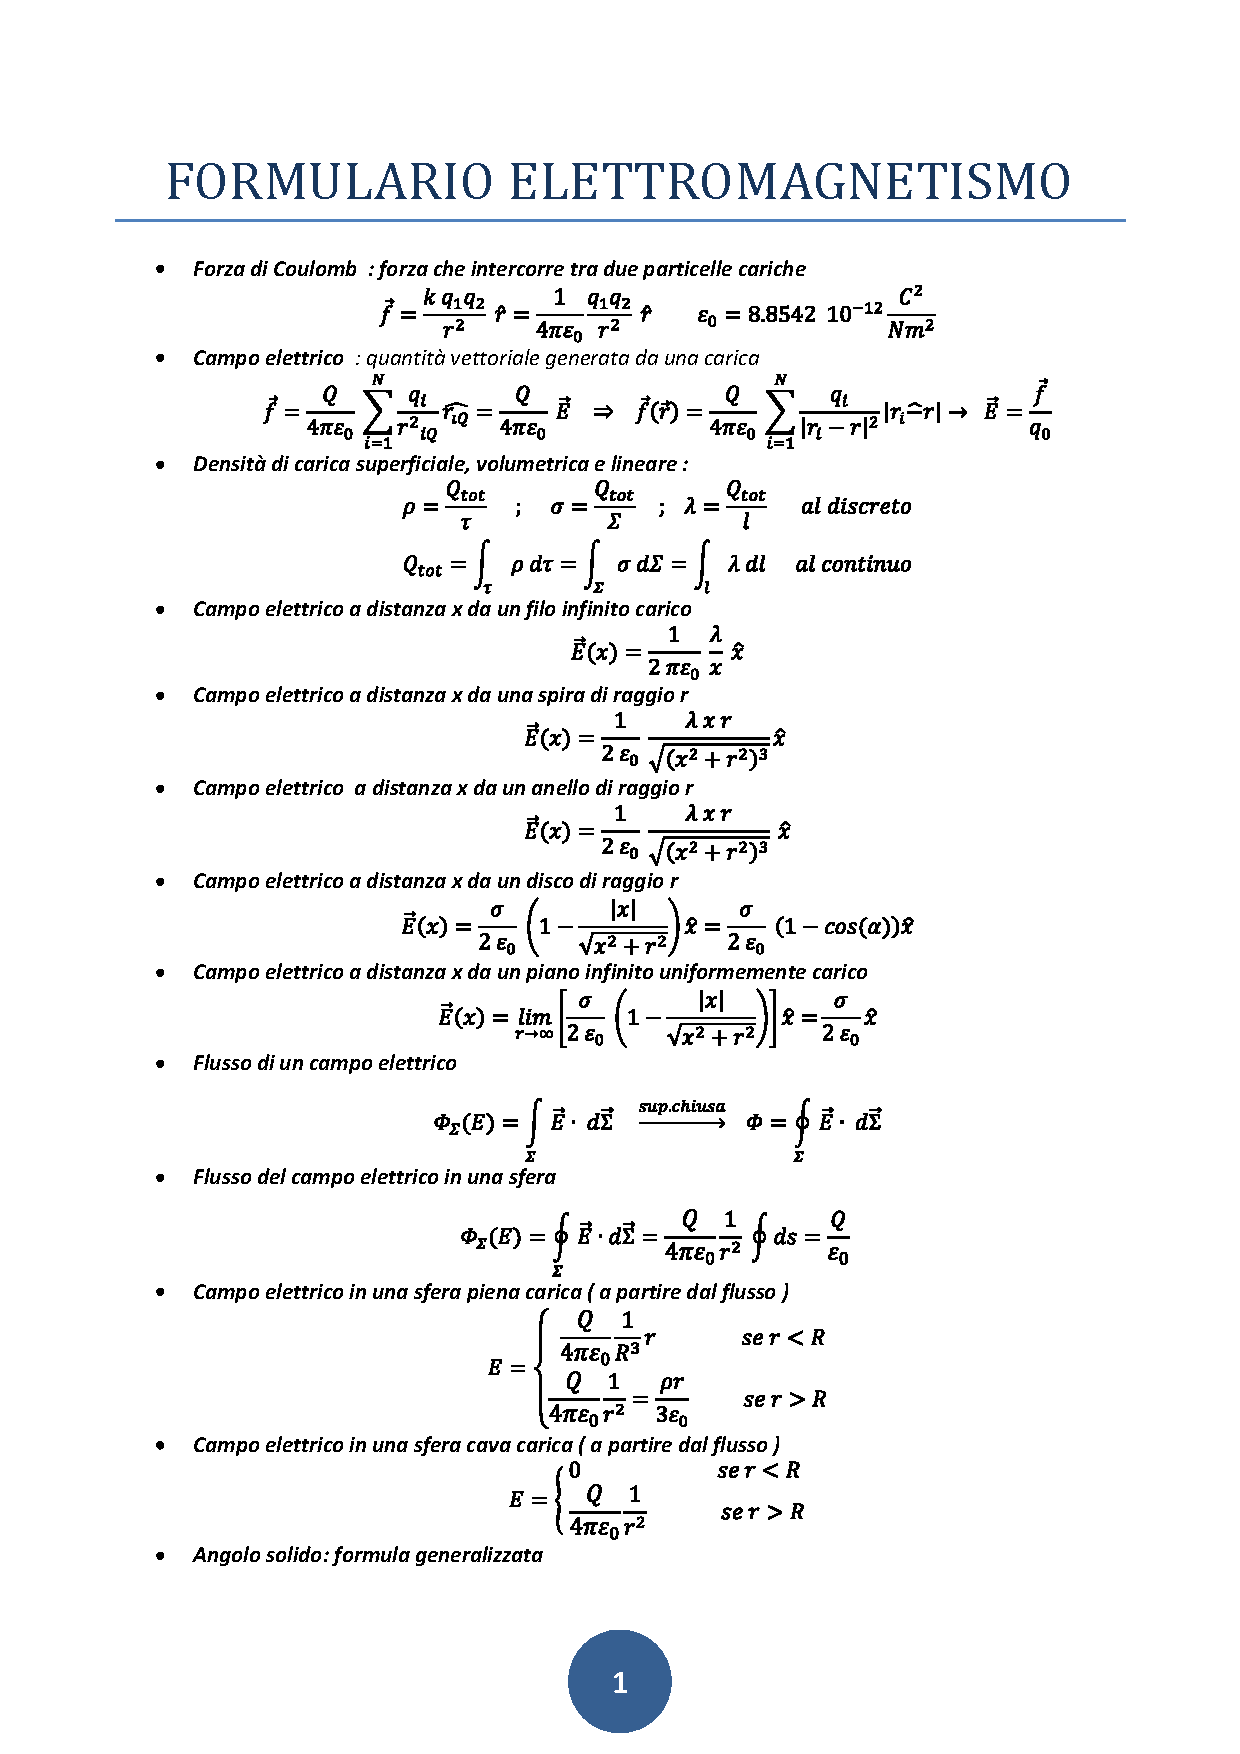
\includepdf[page=-]{Fisica2}
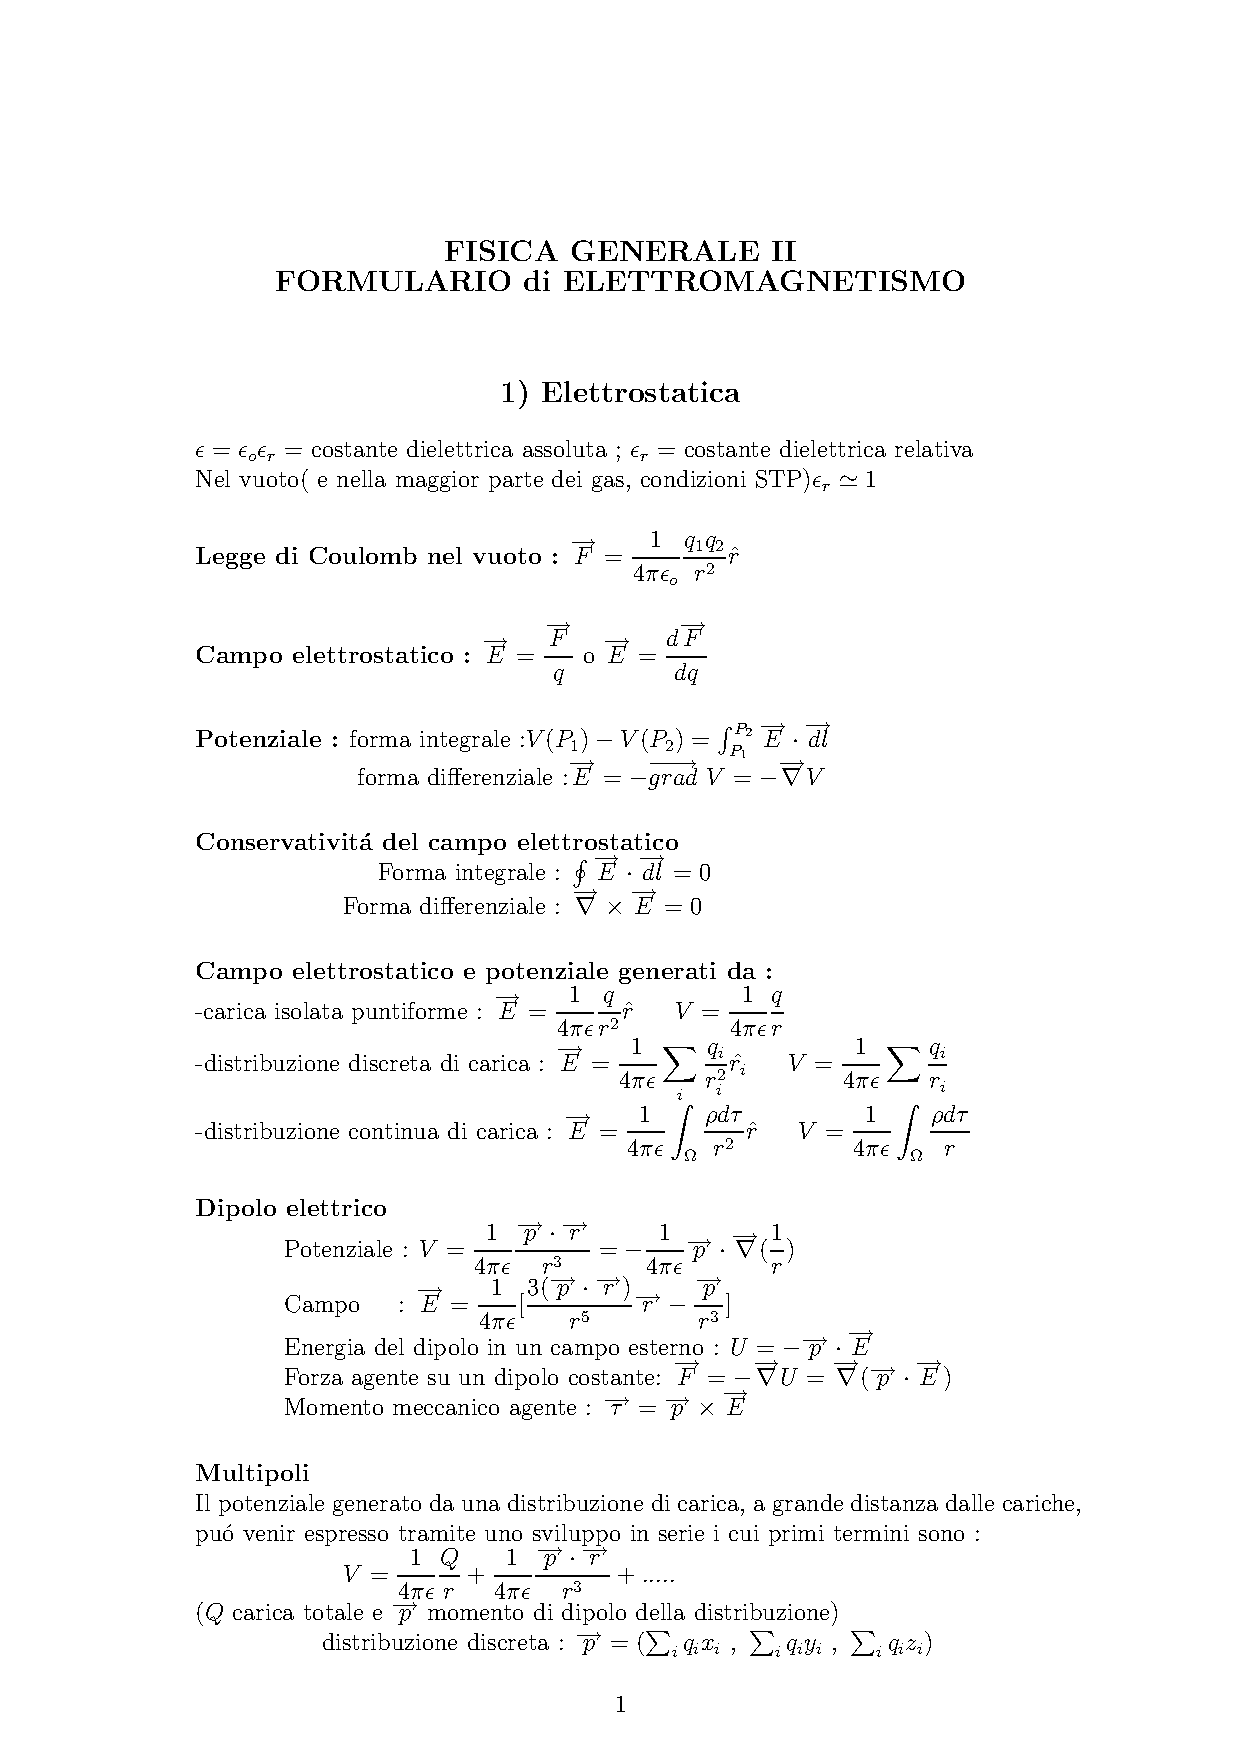
\includepdf[page=-]{Elettro}
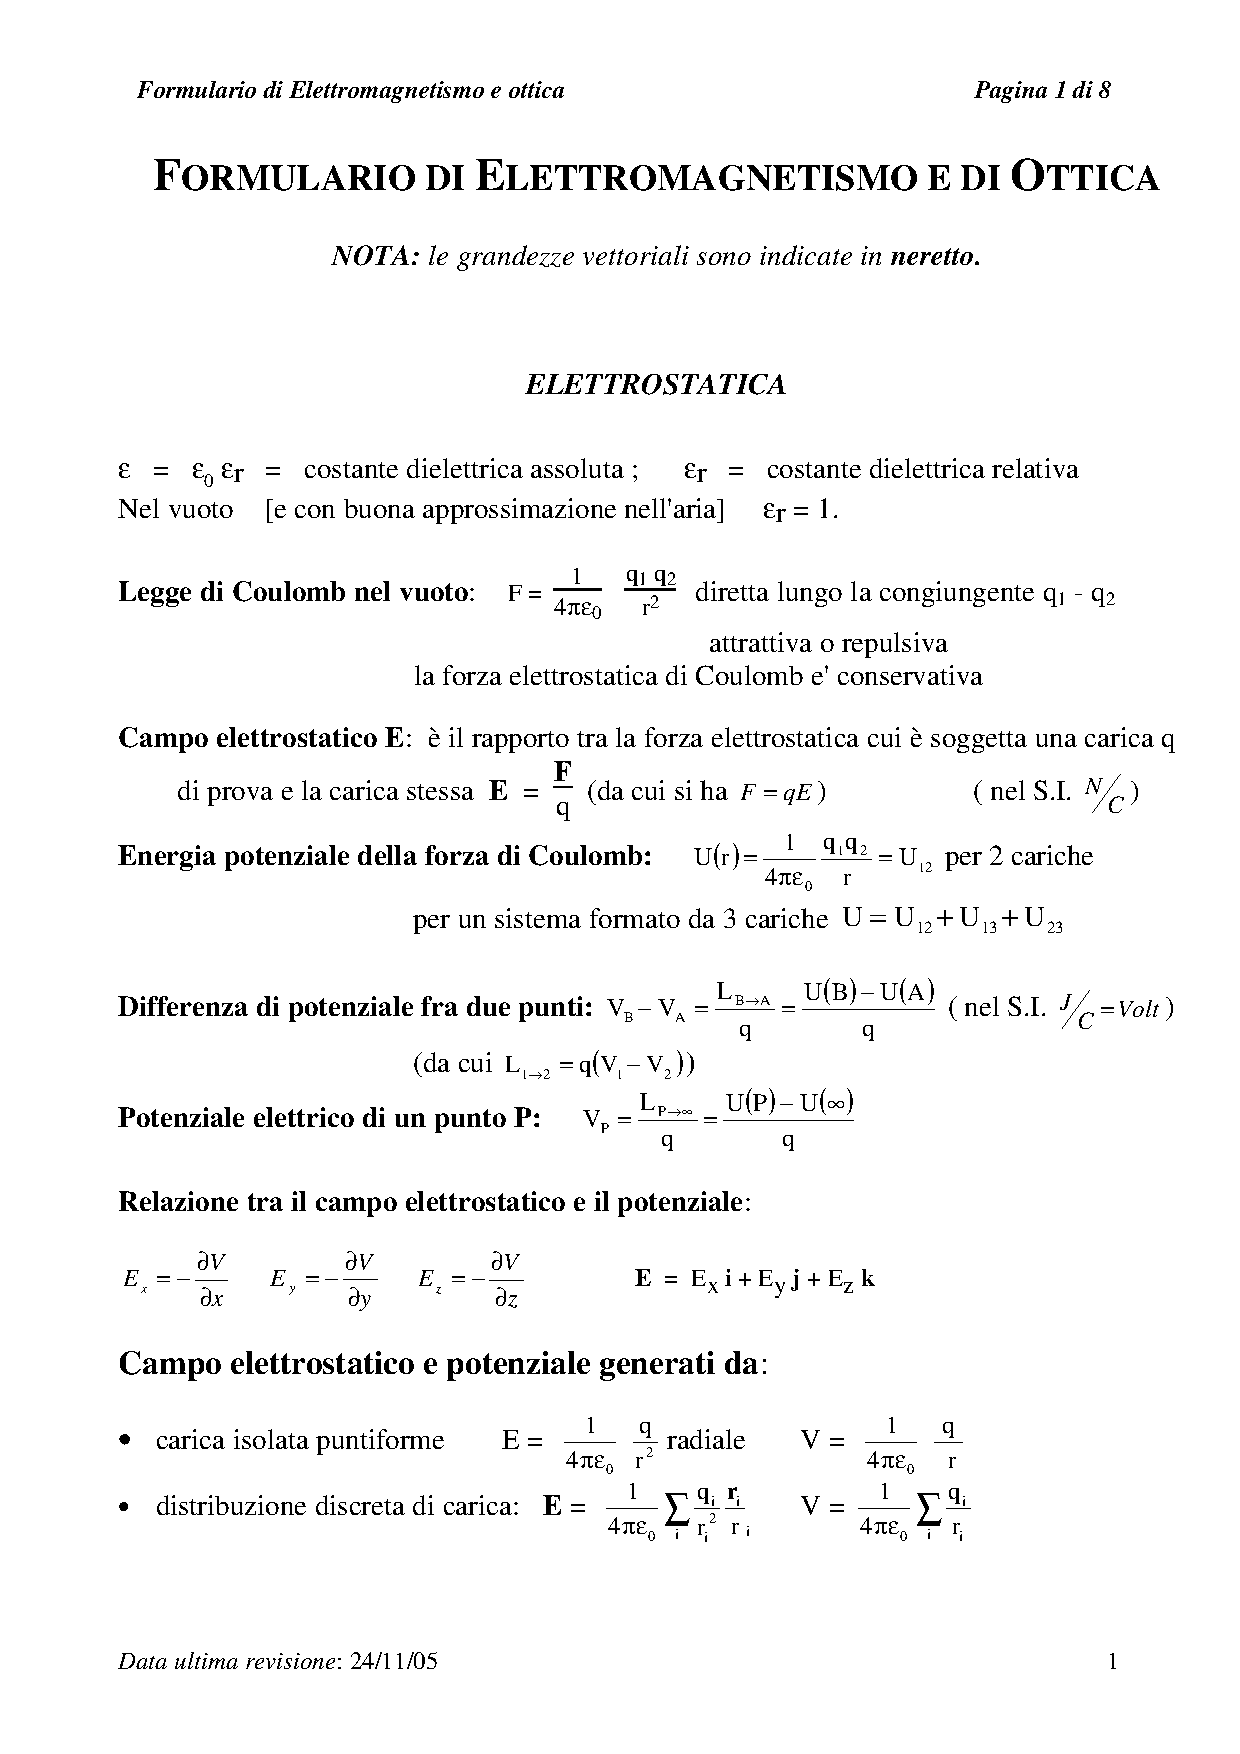
\includepdf[page=-]{Elettroeottica}

\end{document}

\begin{equation*}\begin{split}

\end{split}\end{equation*}